\providecommand{\myrootdir}{..}
\documentclass[\myrootdir/main.tex]{subfiles}

\begin{document}

\chapter{Technique Comparison Study}
\label{sec:study}
\section{Introduction}
To investigate how different factors \todo{do we list these somewhere?} influence BLIRTs we evaluate the three techniques implemented in our tool on the \emph{Failing Build Log Data Set}.

\begin{figure}[h]
	\centering
	\includegraphics[page=6, width=\textwidth, trim={0.5cm 0.5cm 0.5cm 0.5cm}, clip]{img/flow-of-research.pdf}
	\caption{Process of our technique comparison study}
	\label{fig:study}
\end{figure}

\section{Method}
We configure the technique for every example set with an increasing count of I/O examples and then run the retrieval on the next I/O example, the \emph{test I/O example}.
The output from the test I/O example is the oracle for our evaluation.
The examples are sorted and selected chronologically, i.e. the technique is configured with examples from the directly preceeding build logs to extract information from the test log.
The extraction quality of a BLIRT run is evaluated on only one build log, as it should be suitable for every coming example.
Especially the one directly succeeding the configuration.
If the information retrieval there is bad, we expect the user to directly change the configuration again or be dissapointed with his selection of technique.

When evaluating a BLIRT run we measure the following data points:
\begin{itemize}
	\item \textbf{Successful} A BLIRT run is successful when the retrieved output contains all the lines the oracle output.
	\item \textbf{Accuracy} \todo{currently: levenstein difference of input and output, maybe: change to false pos and neg lines}
	\item \textbf{Proximity} \todo{can we usefully calculate that????}
\end{itemize}

taking The Failing Build Log Data Set - run 3(4 with random) techniques with increasing example count - measuring xyz - justify choices like running chronologically / testing on 1 example / no k-fold validation - how are keywords for the search selected?

\section{Results}
\todo{accuracy (or so) of retrievals with growing example number // overall averages \& detailed look on special cases //}
\begin{figure}[hp]
	\centering
	\begin{minipage}{0.45\textwidth}
		\centering
		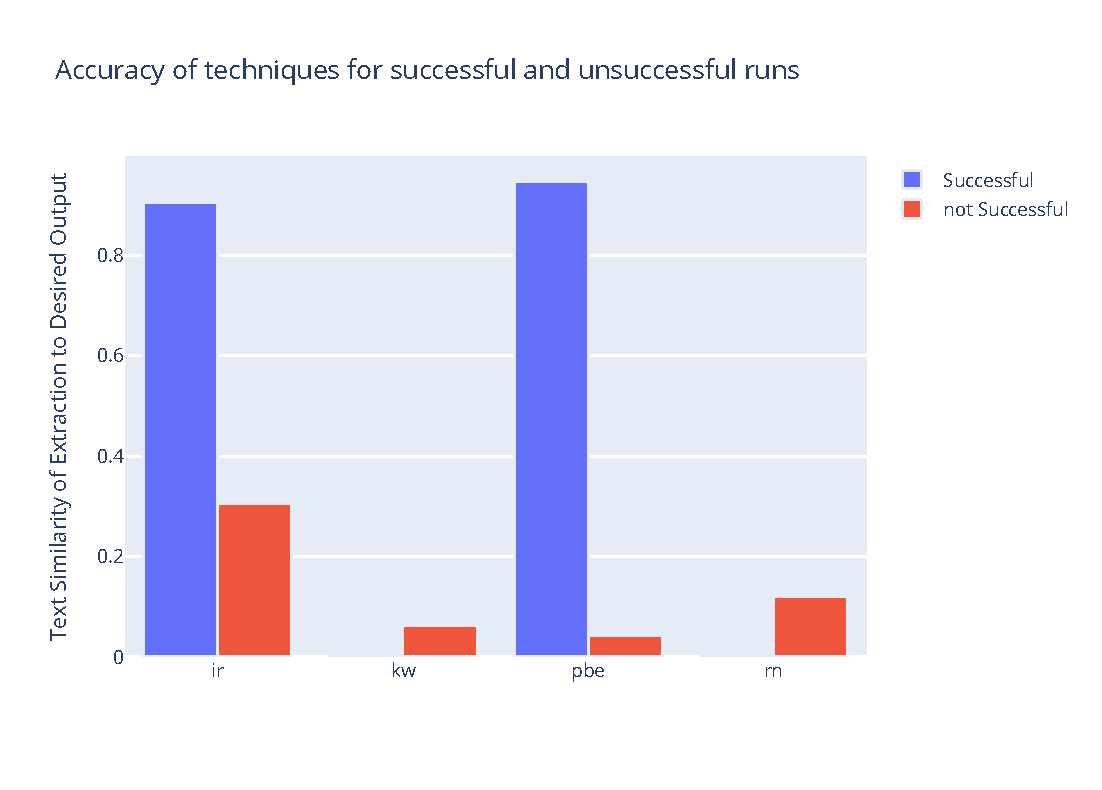
\includegraphics[width=\textwidth, clip]{img/big-study/accuracy-success-all.pdf}
		\caption{caption}
		\label{fig:accuracy-success-all}
	\end{minipage}\hfill
	\begin{minipage}{0.45\textwidth}
		\centering
		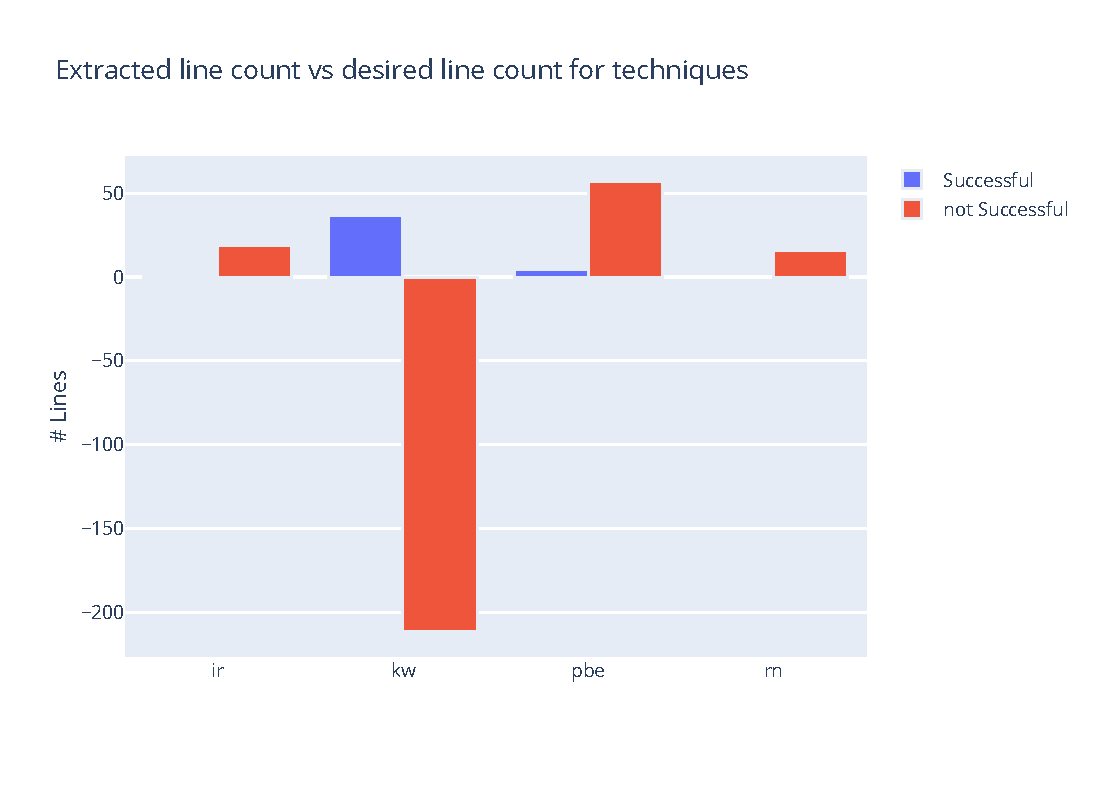
\includegraphics[width=\textwidth, clip]{img/big-study/line-diff-all.pdf}
		\caption{caption}
		\label{fig:line-diff-all}
	\end{minipage}
\end{figure}

\begin{figure}[hp]
	\centering
	\begin{minipage}{0.45\textwidth}
		\centering
		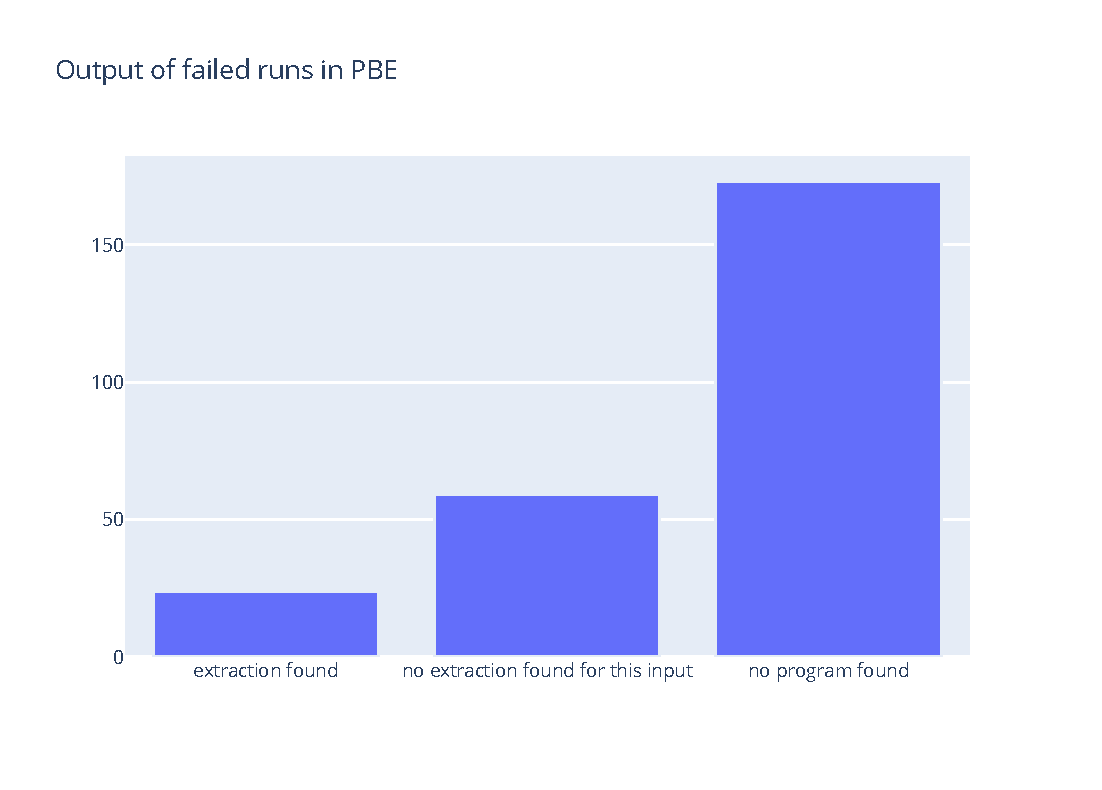
\includegraphics[width=\textwidth, clip]{img/big-study/ouput-failed-pbe.pdf}
		\caption{caption}
		\label{fig:ouput-failed-pbe}
	\end{minipage}\hfill
	\begin{minipage}{0.45\textwidth}
		\centering
		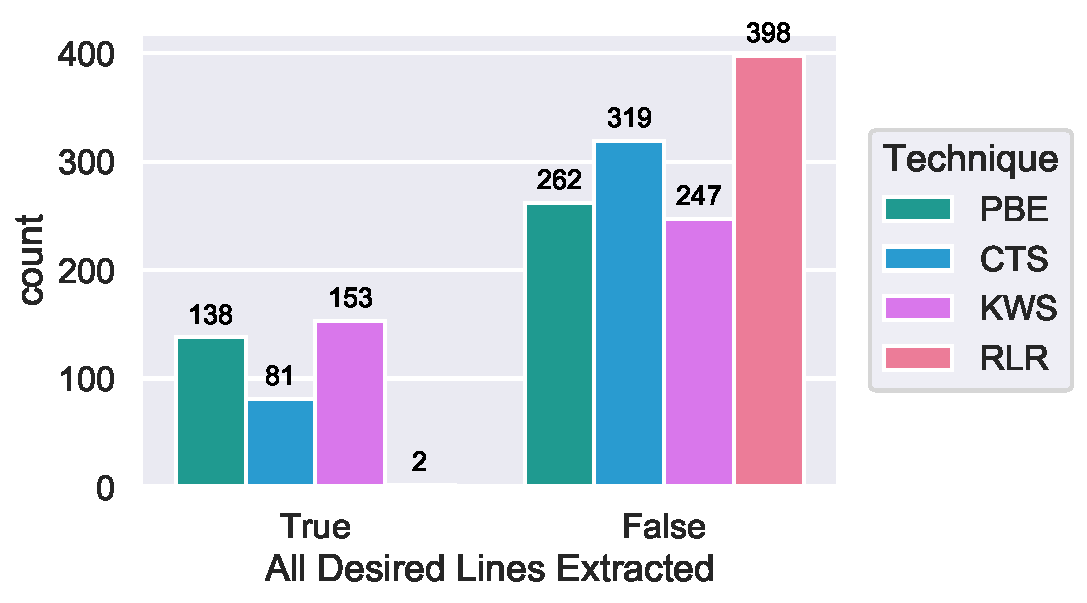
\includegraphics[width=\textwidth, clip]{img/big-study/success-all.pdf}
		\caption{caption}
		\label{fig:success-all}
	\end{minipage}
\end{figure}

\begin{figure}[hp]
	\centering
	\begin{minipage}{0.45\textwidth}
		\centering
		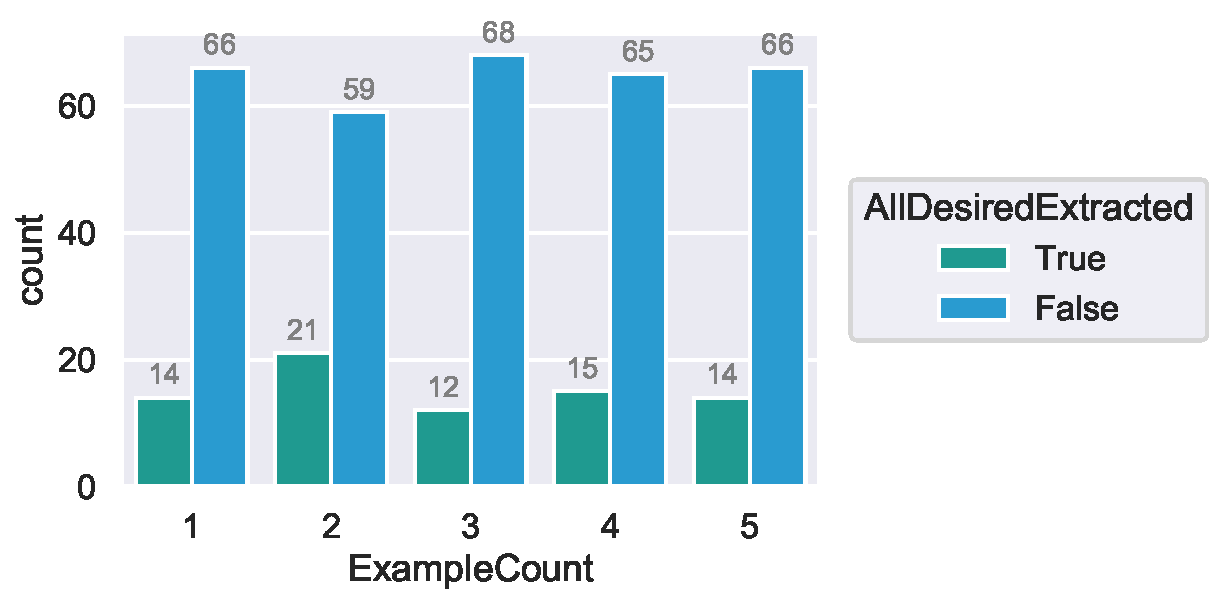
\includegraphics[width=\textwidth, clip]{img/big-study/success-examples-ir.pdf}
		\caption{caption}
		\label{fig:success-examples-ir}
	\end{minipage}\hfill
	\begin{minipage}{0.45\textwidth}
		\centering
		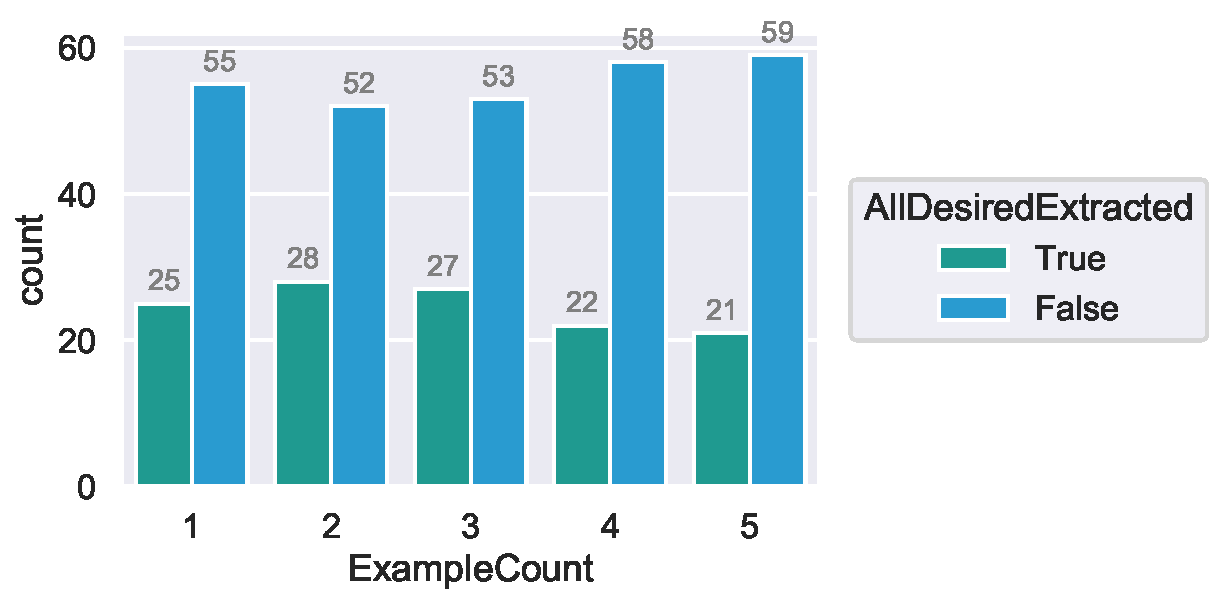
\includegraphics[width=\textwidth, clip]{img/big-study/success-examples-kw.pdf}
		\caption{caption}
		\label{fig:success-examples-kw}
	\end{minipage}
\end{figure}

\begin{figure}[hp]
	\centering
	\begin{minipage}{0.45\textwidth}
		\centering
		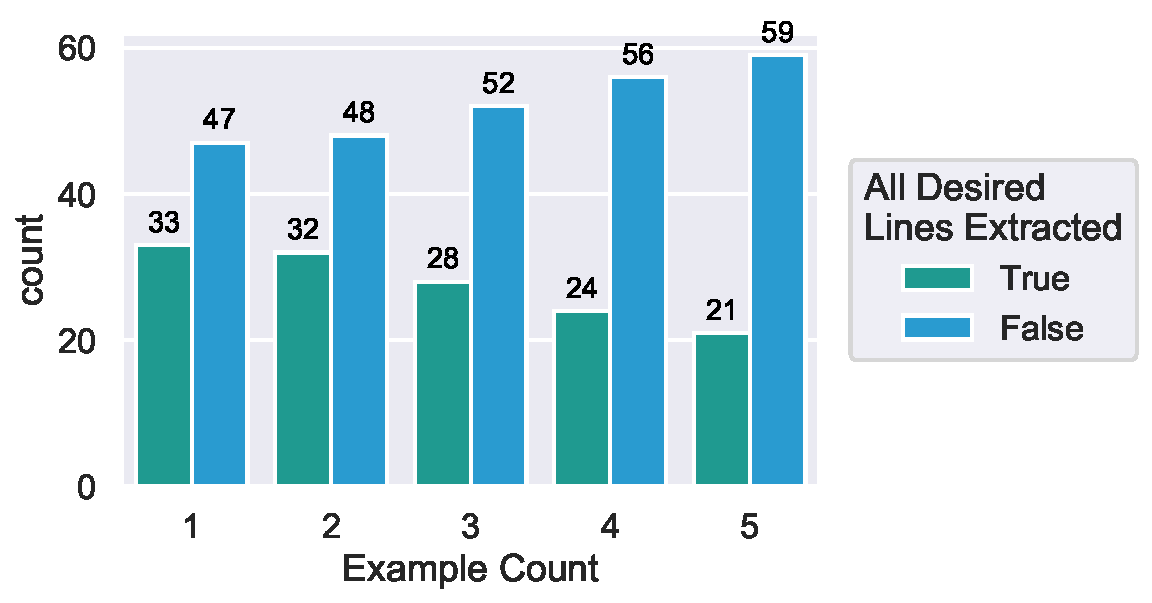
\includegraphics[width=\textwidth, clip]{img/big-study/success-examples-pbe.pdf}
		\caption{caption}
		\label{fig:success-examples-pbe}
	\end{minipage}\hfill
	\begin{minipage}{0.45\textwidth}
		\centering
		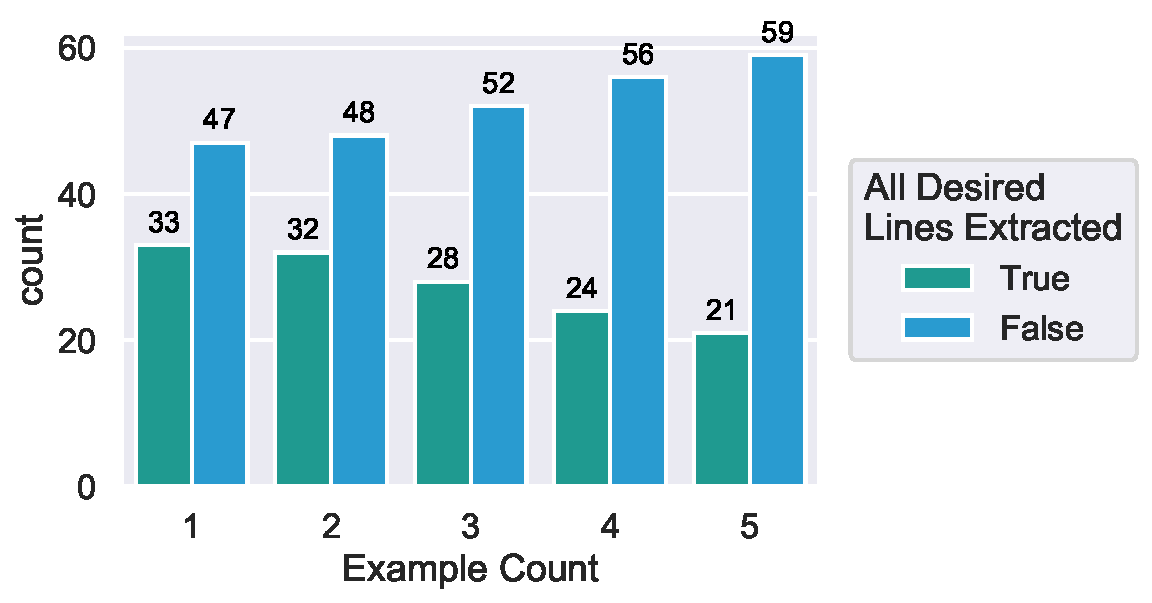
\includegraphics[width=\textwidth, clip]{img/big-study/success-examples-pbe.pdf}
		\caption{caption}
		\label{fig:success-examples-pbe}
	\end{minipage}
\end{figure}

\section{Discussion}
\todo{draw decision tree}

interpret results - when should PROSE be used? - when should text similarity be used? - when should keyword search be used? - answer RQ about PROSE \& other techniques
\section{Threats to Validity}

\end{document}
